% !TEX root = ../main.tex
\chapter{Implementation} % Main chapter title

\label{implementation} % \ref{CHX}


In this chapter we will describe the implementation of the solutions proposed in the previous chapter. Additionally, there will be a comparison between the theoretical solution and the actual implementation as well as a discussion of the difficulties that were encountered during the development process. The chapter is structured according to the previously mentioned main modules of the project: object detection, coordinate transformation, and robotic arm control.
\section{Object detection}

\subsection{First approach}
The first approach to solve the problem of object detection was to use the YOLOv3 model. The model was trained on the COCO dataset, which contains 80 different object classes. During the early stages of development we setup a test scenario in Webots, where we placed various objects in the workspace and used the YOLOv3 model to detect the objects. 

\Vref{fig:object_detection_results} shows the results of the object detection using the YOLOv3 model. The following objects on the workspace are included in the COCO dataset and should therefore be detectable by the model: computer mouse, apple, beer can and orange. The camera perspective in this test scenario was similar to the perspective in the final project setup.  

\begin{figure}[!h]
    \centering
    \adjincludegraphics[width=\textwidth]{Figures/cvResultExistingModel.jpg}
    \caption{Object detection results YOLOv3 model }
    \label{fig:object_detection_results}
\end{figure}


The model was able to detect the beer can with an accuracy of 94 percent. However, the orange only had a likelihood of 71 percent whereas the apple and the computer mouse were not detected at all. Although the model was able to identify the beer can the overall performance was not satisfactory and another solution was needed.

\subsection{Second approach}

The second approach to solve the problem of object detection was to train a custom model. In the project plan, it was not initially planned to train an own model. However, to streamline the process, the decision was made to utilize the ImageAI library, a python library that offers a convenient framework for training and utilizing object detection models. \autocite{ImageAI}

In order to reduce the effort needed to train the model, we decided to use transfer learning, which is a machine learning method where a model, trained on a large dataset, is used as a starting point for a new model. The new model is then trained, containing the pre-trained weights of the origin model. \autocite{mlearning} We chose to use the pre-trained YOLOv3 model, mentioned above, as the basis for transfer learning. 

\subsection{Training data }

The first step to train a custom model is to gather and arrange the training data in the YOLO annotation format. In this format the data is divided into two main directories: "train" and "validation". Each of these directories contains two sub-directories: "images" and "annotations". It's recommended to use 80\% of the data for training and 20\% for validation. The data consists of both images of objects we want to detect and accompanying annotation files. Each image is linked with a corresponding annotation file that shares the same name as the image file and provides information about the objects in the image. The general structure of the object annotation is shown below. 

\begin{lstlisting}[language=prolog]
<object-class><x-pos><y-pos><width><height>
\end{lstlisting}

The file contains one line for each object in the image. The object class is an integer that represents the type of the object. The value corresponds to a list of objects in another file named "classes.txt" inside the "annotation" directory and is encoded by the index of the object in the list. The x-pos, y-pos, width, and height are the information for the bounding box of the object in the image. The values are normalized to the range [0, 1] and are relative to the width and height of the image.

\subsubsection{Automatization}

Instead of creating and labeling the images manually we decided to automate the process. The plan was to utilize the object detection feature integrated in Webots to automatically generate the image and annotation files within their respective directories. We only utilized this detection method to create training data, as the detection is not based on image recognition but hard coded within Webots. 

Two configurations were set up to generate training data. The first setup produces data with a top-down camera view and multiple objects arranged on the table. The second setup generates images with individual objects positioned on the table at different orientations and rotated camera at four distinct viewpoints.

\subsubsection{Configuration 1: Top down}

The initial step in realizing the top-down configuration involved the definition of a function for capturing camera images and generating the corresponding annotation files. This function utilizes a reference of the camera object to obtain the objects currently detected, determine the values needed for annotation and store the images in their designated directories. The following code segment demonstrates a shortened version of the implementation of this function.

\begin{lstlisting}[language=python]
def createTrainingFiles(camera,type = "train"):
   ... # initialize variables and generate pathes
   while True: # get current fileName
      filename = f"image_{fileNamePostfix}.txt"
      filepath = os.path.join(annotationPath, filename)
      if not os.path.isfile(filepath): 
          break # if file does not exist, use this name
      fileNamePostfix += 1
  fileName = f"image_{fileNamePostfix}"
  for obj in recognizedObjectes:
      id = obj.getId()
      name = obj.getModel()
      if name not in categories:
          continue
      position = list(obj.getPosition())
      positionOnImage = list(obj.getPositionOnImage())
      orientation = list(obj.getOrientation())
      size = list(obj.getSize())
      sizeOnImage = list(obj.getSizeOnImage())
      relativeSize = [sizeOnImage[0]/imageWidth, sizeOnImage[1]/imageHeight]
      relativePosition = [positionOnImage[0]/imageWidth, positionOnImage[1]/imageHeight]
      yoloData.append(f"{categories.index(name)} {relativePosition[0]} {relativePosition[1]} {relativeSize[0]} {relativeSize[1]}\n")
      jsonData.append({
          "id": id,
          ... # adding the remaining properties to json data
      })
  camera.saveImage(imagePath+fileName+".jpg",100) # save image
  with open(jsonPath+fileName+".json", 'w') as file: # save json data
      json.dump(jsonData, file, indent=4)   
  with open(annotationPath+fileName+".txt", 'w') as file: # save yolo annotation
      file.writelines(yoloData)
\end{lstlisting}
The function accepts two parameters, a reference to the camera object, and a "type". The purpose of the "type" parameter is to specify whether the function should generate training or validation data. The function starts by initializing various variables and generating file paths for the image, annotation, and JSON data. In addition to the required training data, all available information about an object was saved in a JSON file so that it can be used later. The JSON file shares the same name as the image file and is stored in the directory \(raw\_data\). Lines 3-8 determine the current file name for the output files. The filename is generated by appending a postfix to the string \(image\). The postfix is generated by incrementing a counter until a file with the generated name does not exist. This ensures that the file name is unique and does not overwrite existing files.
At line 10 a loop iterates over the objects that the camera recognizes, and collects information about each object, including its model name, position and size. These values are converted into the required format, by determining the object's relative position and size. Subsequently, in lines 22 and 23, strings for the annotation and the JSON representation of the detected object are prepared so they can be appended to the corresponding lists for this image. Finally, the function saves the image, JSON data, and YOLO annotation data to their respective files using the file name generated earlier. The image is saved using the camera's "saveImage" function.

After a snapshot was taken the object's position and orientation on the table needed to be randomized. The function to realize the object randomization is shown below.

\begin{lstlisting}[language=python]
def moveTableNodes(supervisor,table):
   margin = 0.1
   bottomLeft = table.local2world([0,1,0])
   topRight = table.local2world([1,0,0])
   x_min = bottomLeft[0] + (topRight[0] - bottomLeft[0]) * margin
   x_max = topRight[0] - (topRight[0] - bottomLeft[0]) * margin
   y_min = bottomLeft[1] + (topRight[1] - bottomLeft[1]) * margin
   y_max = topRight[1] - (topRight[1] - bottomLeft[1]) * margin
  for cat in categories:
       obj = supervisor.getFromDef(cat)
       x = random.uniform(x_min, x_max)
       y = random.uniform(y_min, y_max)
       z = bottomLeft[2] # any z coordinate
       obj.getField('translation').setSFVec3f([x, y, z])
       xRotation = random.uniform(1, 360)
       yRotation = random.uniform(1, 360)
       zRotation = random.uniform(1, 360)
       angle = random.uniform(1, 360)
       obj.getField('rotation').setSFRotation([xRotation,yRotation,zRotation,angle])

\end{lstlisting}
The function accepts two parameters: a reference to the supervisor object and a reference to the table object. The method begins by determining the boundaries of the table using coordinate transformation. Intervals for the x and y coordinates are determined for the random positioning of objects on the table and then adjusted to leave a margin of 0.1 meters around it. At line 9 a loop iterates the objects on the table and generates a random position and orientation for each object using the previously calculates intervals.

Finally a loop needed to be developed to call the snapshot and object randomization functions a specified number of times with a certain delay between each iteration. A decorator was used to extend the function to be repeatedly called until a specified condition is met while advancing the simulation. The following code segment demonstrates the implementation of this loop. 

\begin{lstlisting}[language=python]
@looper
def randomPosSamplingLoop(self,sampleSize,type):
    if self.loopCount % 10 == 0:
        if self.loopCount % 20 == 0:
            TrainingsHelper.moveTableNodes(self.supervisor,self.mainTable)
        else:
            TrainingsHelper.makeSnapshot(self.camera,type)
            self.dataCount +=1
    self.loopCount += 1
    if self.dataCount>sampleSize:
        return -1
\end{lstlisting}
The function takes two arguments as input: the quantity of samples, and the type of data, to be generated. In operation, the function initiates the execution of the \(moveTableNodes\) function at regular intervals of 20 iterations, ensuring the repositioning and reorientation of the objects every 2 seconds. Additionally, the \(makeSnapshot\) function is called every 10 iterations to secure the capturing of snapshots at a rate of once per second. The function concludes its operation by returning a value of -1 when the predetermined number of samples has been generated.

The method must be invoked twice, once for the generation of training data and once for the generation of validation data. Upon the completion of this process, a dataset is produced that is ready for the training of a custom model. \Vref{fig:dataset_train_img} and \Vref{fig:dataset_train_ann} present a dataset sample, generated by with this configuration, containing the image and its accompanying annotation file.

\begin{figure}[!h]
    \centering
    \adjincludegraphics[width=\textwidth]{Figures/image_344.jpg}
    \caption{image\_344.jpg in image directory  }
    \label{fig:dataset_train_img}
\end{figure}

\begin{figure}[!h]
    \centering
    \adjincludegraphics[width=\textwidth]{Figures/image_344.txt.jpg}
    \caption{image\_344.txt in annotations directory  }
    \label{fig:dataset_train_ann}
\end{figure}

We generated 1200 images for training and 300 images for validation using this configuration. In order to enhance the performance of the model, an alternative image configuration was also developed.

\subsubsection{Configuration 2: Four-angled rotation}

The second configuration was designed to provide single object images at four distinct viewpoints, serving as training data. To achieve this, a function was created to relocate the camera to a designated viewpoint. This function accepts two inputs: a reference to the supervisor object and an index specifying the desired viewpoint. The supervisor is used to alter the camera perspective while index is utilized to determine the camera's position based on a list of coordinates. Furthermore, a function was implemented to facilitate the exchange of objects on the table. This function takes three inputs as arguments: a reference to the supervisor object, a reference to the table object, and an index indicating the desired object. Finally, a function was created to randomly modify the orientation of the current node-object, resulting in a diverse set of images taken from the same viewpoint. After the completion of these steps, a routine was implemented that integrates the various functions. The code segment below presents the implementation of this function. 

\begin{lstlisting}[language=python]
def single_objectImage_setup(supervisor,table,imagesPerViewpoint):
    global count, currentNode, lastViewPointPos
    amountViewpoints = 4
    if(count==0): # init viewpoint position for first run
        moveViewPoint(supervisor,lastViewPointPos)
        swapObj(currentNode,table,supervisor)
    # change viewpoint if given imagesPerViewpoint is met
    if((count % imagesPerViewpoint) == 0):
        lastViewPointPos = (lastViewPointPos+1)%4
        moveViewPoint(supervisor,lastViewPointPos)
    # change object if limit is met
    if((count % (imagesPerViewpoint*amountViewpoints))==0):
        currentNode = (currentNode+1) % len(categories)
        swapObj(currentNode,table,supervisor)
    spinTableNode(supervisor,table,currentNode)
    count += 1
\end{lstlisting}
The function is meant to be executed each time after an image has been created and prepares the next image to be captured. The number of image configurations provided by the function is determined by the value of "imagesPerViewpoint". A global variable is used to keep track of the number of function invocations. The first time this method is called, the viewpoint and the first object are initialized. The if statement at line 8 verifies whether the number of images taken from the current viewpoint has reached the predetermined limit. In the event that the limit has been met, the viewpoint is shifted to the next one in the designated list. At line 12, the an if statement determines whether the number of images captured from the current object has reached its limit. If this is the case, the object is swapped for the next one in the list. Finally, the function rotates the current object to a random orientation with each invocation. 

The training data can be generated using the same function as in the first configuration. The loop to call these functions during the simulation closely mirrors the looper-function used before. The code segment below demonstrates the implementation of the method. 

\begin{lstlisting}[language=python]	
@looper
def singleObjectImageLoop(self,imagesPerPerspective,type):
    if self.loopCount % 10 == 0:
        if self.loopCount % 20 == 0:
            TrainingsHelper.single_objectImage_setup(self.supervisor,self.mainTable,imagesPerPerspective)
        else:
            TrainingsHelper.makeSnapshot(self.dataCam,type)
            self.dataCount +=1
    self.loopCount += 1
    if self.dataCount>imagesPerPerspective*amountPerspectives*len(categories): 
        return -1
\end{lstlisting}

This loop operates similar to the first configuration, alternately executing the \(single\_object\_setup\) and \(makeSnapshot\) functions with a set time delay. The termination criteria for this loop has been revised to ensure that the number of iterations is equal to the product of the amount of images per perspective, the number of perspectives, and the number of objects. In this configuration, we generated 256 training images and 64 validation images per object, capturing diverse orientations of the object from 4 different viewpoints.

\subsection{Training }

A total of 1456 images were generated for training and 384 images for validation. The training was performed using the ImageAI library, which provides a pre-trained YOLOv3 model that was used as a starting point for transfer learning. The following code segments presents the implementation of the training function, using the ImageAI library. 

\begin{lstlisting}[language=python]
def startTraining():
    execution_path = os.path.dirname(__file__)
    data_dir_path = os.path.join(execution_path , "DataSet")
    model_path = os.path.join(execution_path , "Modelle/yolov3.pt")
    createClassFiles(categories) 
    trainer = DetectionModelTrainer()
    trainer.setModelTypeAsYOLOv3()
    trainer.setDataDirectory(data_directory=data_dir_path)
    trainer.setTrainConfig(object_names_array=categories, batch_size=32, num_experiments=100, train_from_pretrained_model=model_path)
    trainer.trainModel()
\end{lstlisting}
The function sets up the data directory, model path, and configuration for the training process. It also creates the class files for the categories to be detected and initiates the training process using the "trainModel" method. The "DetectionModelTrainer" class from the ImageAI library is used to set up and train the model, with parameters such as batch size, number of training experiments, and object categories specified. 

The batch size was set to 32, while the number of training iterations through the dataset was set to 100. The training process was performed on a desktop computer using a NVIDIA GeForce RTX 4080 graphics card, an AMD Ryzen 7 5800X3D processor and 32 GB of ram. The training process took approximately 8 hours to complete.


\subsection{Result }

The results of the training after the 100th iteration are presented below.

\begin{lstlisting}[language=python]
    recall: 0.748433 precision: 0.683522 mAP@0.5: 0.736085, mAP@0.5-0.95: 0.340358
\end{lstlisting}

The results of the evaluation revealed that the model achieved a recall value of 0.748433, precision value of 0.683522, mAP@0.5 value of 0.736085, and mAP@0.5-0.95 value of 0.340358. 

The recall value of 0.748433 indicates that the model correctly detected 74.84\% of all positive instances present in the test dataset. Precision measures the proportion of detected instances that were correctly identified as positive. The precision value of 0.683522 suggests that 68.35\% of the instances detected by the model were positive. The mAP (Mean Average Precision) metric is a measure of accuracy in object detection tasks. The mAP@0.5 value of 0.736085 indicates that, on average, the model achieved a precision of 73.60\% in detecting objects in the test dataset, with a threshold of 0.5 for Intersection over Union (IoU) between the ground-truth and predicted bounding boxes. The Intersection over Union is a metric used to evaluate the similarity between two bounding boxes and measures the ratio of the area of intersection between the two boxes to the area of their union. Similarly, the mAP@0.5-0.95 value of 0.340358 suggests an average precision of 34.03\% in detecting objects using a range of IoU thresholds from 0.5 to 0.95. 

The low mAP@0.5-0.95 score indicates that the model is more likely to detect multiple bounding boxes for the same object with a high probability. \Vref{fig:trained_model_results} shows the results of the object detection process using the custom model and demonstrates the problem. 

\begin{figure}[!h]
    \centering
    \adjincludegraphics[width=\textwidth]{Figures/snapshot-detected-nms0.5.jpg}
    \caption{Object detection results self trained model }
    \label{fig:trained_model_results}
\end{figure}

Multiple bounding boxes with high probabilities were created respectively for each object, leading to distorted results, which is a common problem in object detection tasks. One possible reason for this issue could be overfitting, where the model has been trained for an extended period and has memorized the training data. Another possible cause could be an insufficient training dataset, which lacks diversity in its data, as it only provides a limited number of image configurations, despite the dataset's scope being sufficient.

The problem can be addressed by using non-maximum suppression (NMS) to find the best fitting box based on a given threshold. The NMS algorithm is implemented in the ImageAI library and can be used by setting the \(nms\_threshold\) parameter in the corresponding function. The NMS threshold is used to determine when two bounding boxes should be considered duplicates and only one should be kept. If the overlap between two bounding boxes, measured by the IoU, is greater than or equal to the NMS threshold, then  the bounding boxes with the lower confidence score will be eliminated alternatively both bounding boxes will be kept, as they are considered to be separate detections. By setting the NMS threshold to a certain value, the algorithm can eliminate duplicates and produce a cleaner, more accurate output. 

The results of the object detection process using The NMS algorithm with a threshold of 0.05 are presented in \vref{fig:trained_model_results_2}.

\begin{figure}[!h]
    \centering
    \adjincludegraphics[width=\textwidth]{Figures/snapshot-detected.jpg}
    \caption{Object detection results self trained model }
    \label{fig:trained_model_results_2}
\end{figure}

The test results indicate that the model has a satisfactory level of performance for the intended application, as it was capable to correctly determine the position and class of each object on the table in multiple test cases. 

To use the model during simulation a class was implemented to handle the object detection process. The class contains a method to detect objects in a given image, returning a list of detections and their respective bounding boxes as well as the corresponding orientation.

\section{Orientation of the object}

To determine the angle of an object relative to the table, the cv2 library was utilized. The approach relies on Principle Component Analysis (PCA) to determine the primary orientation of the object's contours. The function used to prepare the image for the orientation analysis is presented below.

\begin{lstlisting}[language=python]
def getAngle(self, objectImage, name: str|None = None, savefig: bool|None = None) -> float:
        try:
            # (1) Image of object is cropped using the bounding box and passed as a parameter
            # (2) Convert the image to the HSV color space
            hsv_image = cv2.cvtColor(objectImage, cv2.COLOR_BGR2HSV)
            # (3) Apply Canny edge detection
            edges = cv2.Canny(hsv_image, 50, 150)
            # Init masks
            leftEdgeMask=np.full(np.shape(edges),0)
            rightEdgeMask=np.full(np.shape(edges),0)
            topEdgeMask=np.full(np.shape(edges),0)
            bottomEdgeMask=np.full(np.shape(edges),0)
            # Init Boundary
            leftEdge=[1000 for i in range(np.shape(edges)[0])]
            rightEdge=[0 for i in range(np.shape(edges)[0])]
            topEdge=[1000 for i in range(np.shape(edges)[1])]
            bottomEdge=[0 for i in range(np.shape(edges)[1])]
            # Position Boundary
            for y,x in pos:
                leftEdge[y] = min(leftEdge[y],x)
                rightEdge[y] = max(rightEdge[y],x)
                topEdge[x] = min(topEdge[x],y)
                bottomEdge[x] = max(bottomEdge[x],y)
            # Make Masks from Boundary
            for y,x in enumerate(leftEdge):
                leftEdgeMask[y,x:] = 255
            for y,x in enumerate(rightEdge):
                rightEdgeMask[y,:x] = 255
            for x,y in enumerate(topEdge):
                topEdgeMask[y:,x] = 255
            for x,y in enumerate(bottomEdge):
                bottomEdgeMask[:y,x] = 255
            # (4) Remove inner edges by applying a mask to the image
            combined_mask = (leftEdgeMask*rightEdgeMask*bottomEdgeMask*topEdgeMask/255**3)
            # (5) Applying gaussian blur to smoothen edges
            blur = cv2.GaussianBlur(combined_mask, (11,11), 0)
            # (6) Using canny algorithm again to detect contours
            cleanEdges = cv2.Canny(blur.astype('uint8'),50,150)
            # (7) Using PCA (Principal Component Analysis) to compute the main orientation of the object
            orientation, contourNangle = self.getOrientationPCA(cleanEdges,objectImage)
            return orientation
\end{lstlisting}

The first step is to crop an image of the object using the bounding box coordinates provided by the object detection class. The image is then converted to the HSV color space and edges are detected using the Canny algorithm from the OpenCV library. The next step is to remove the object's inner edges by applying a mask to the image. This mask is created by selecting all the pixels that do not have any edge pixels between itself and at least one of the image's borders.

The edges are then smoothed using a Gaussian blur and contours are detected using the Canny algorithm a second time. Finally, the main orientation of the object is computed using the function "getOrientationPCA", presented in the following code segment.

\begin{lstlisting}[language=python]
def getOrientationPCA(self, edges):
    pts = np.transpose(np.where(edges>1),[1,0]).astype(np.float64)
    # Perform PCA analysis
    mean = np.empty((0))
    mean, eigenvectors, eigenvalues = cv2.PCACompute2(pts, mean)
    angle = math.atan2(eigenvectors[0,1], eigenvectors[0,0]) # orientation in radians
    return angle
\end{lstlisting}
This approach to determining the orientation of an object is based on the assumption that the main orientation of an object can be determined by finding the eigenvector with the highest variance in the dataset of edge points. OpenCV's principal component analysis implementation is used to find the eigenvectors of the dataset. The angle to the x-axis of the eigenvector with the highest variance is then calculated and returned as the main orientation of the object. The implementation of the function is partially based on an implementation example. \autocite{orientation}

A graphical representation of these steps is shown in \vref{fig:orientation_steps}, which highlights the individual images of the object at different stages of the process. 

\begin{figure}[!h]
    \centering
    \adjincludegraphics[width=\textwidth]{Figures/hammerTime.jpg}
    \caption{Steps do determine the orientation of an object }
    \label{fig:orientation_steps}
\end{figure}

The annotations below the images correspond to the respective steps in the "getAngle" function and are referred to in the comments of the function.

The first image corresponds to the original cropped section containing the object of interest. The second image displays the result obtained by performing a conversion to the HSV color space. This was performed to improve the distinction of edges between areas with different hues. Applying the Canny algorithm to this produces the third image as a result. The fourth image shows the area obtained by selecting all the pixels not encased by the detected edges. Applying a gaussian blur to this results in smoother edges as can be seen in the fifth image. Performing a second pass of the Canny algorithm results in what can be seen in the sixth image. Lastly, the seventh image shows the original cropped section of the object with an overlay displaying the direction of the eigenvectors, which determines the rotation of the object in relation to the fixed coordinate system of the image.

\section{Coordinate transformation}

With relative position of the objects within the image, this position vectors need to be transformed to the world coordinate system to know their position in the simulation relative to the robot. 
This task was achieved by creating and combining two transformation matrices. The general procedure was implemented as follows:


\begin{lstlisting}[language=python]
# Transformation Matrix from table corner in image to table center
# - Rotation and Translation Matrix
img2table_rot_trans = [[0, -1,  0, 0.5],
                      [-1,  0,  0, 0.5],
                      [ 0,  0, -1,   1],
                      [ 0,  0,  0,   1]]

# - Scaling Matrix
img2table_scale = [[Table.size[0],             0,             0,  0],
                   [            0, Table.size[1],             0,  0],
                   [            0,             0, Table.size[2],  0],
                   [            0,             0,             0,  1]]

# Transformation Matrix from image to table center
img2table = numpy.matmul(img2table_scale, img2table_rot_trans)

# Transformation Matrix from table center to world
table2world = numpy.array([[cos(Table.rotation[3]), -sin(Table.rotation[3]),  0,  Table.position[0]],
                           [sin(Table.rotation[3]),  cos(Table.rotation[3]),  0,  Table.position[1]],
                           [                     0,                       0,  1,  Table.position[2]],
                           [                     0,                       0,  0,                 1]])

# Transformation Matrix from image to world
TMatrix = numpy.matmul(table2world, img2table)
\end{lstlisting}

Since the origin of the table's coordinate system is in the center of the table and therefore the table's position and orientation reference its center point, a translation needs to be applied to the position vector in the image, whose coordinate system is located on the top left corner, while also rotating the coordinate axes to match the ones of the table's origin.

A second matrix is then used to scale the position vector to the dimensions of the table with the help of the Table's properties supplied by the webots API.

The rotation and translation matrix $\mathbf{M_{rt}}$ is then multiplied with the scaling matrix $\mathbf{M_s}$ to produce the transformation matrix $\mathbf{M_{img2table}}$ from the image coordinate system to the table coordinate system.

$$\mathbf{M_{img2table}} = \mathbf{M_s} \cdot \mathbf{M_{rt}}$$

\textcolor{red}{Figure X shows the coordinate systems of the image and table relative to eachother the vectors for a point in each of them. Shows the result of applying the first Transformation matrix to a point in the image} % end red


A second transformation matrix is then responsible for transforming the position vector from the table coordinate system to the world coordinate system. For this implementation, a level table surface parallel to the XY plane is assumed, only allowing a rotation of the table in the Z axis. The rotation matrix is created from the rotation vector of the table, and the translation is taken from its position vector relative to the world origin, resulting in the transformation matrix $\mathbf{M_{table2world}}$.

These two transformation matrices are then multiplied with one another to produce a final transformation matrix $\mathbf{M_{img2world}}$ in order to directly transform the position vector from the image coordinate system to the world coordinate system.

$$\mathbf{M_{img2world}} = \mathbf{M_{table2world}} \cdot \mathbf{M_{img2table}}$$



\textcolor{red}{ Gotta mention the Z axis is flipped in the image coordinate system } % end red
\textcolor{red}{ Include sample code to perform actual conversion, adding a fourth value to the position vector} % end red

% <!-- 
%  This matrix is created by multiplying the position vector with the rotation matrix $M_r$ and the translation matrix $M_t$ to produce the final transformation matrix $M_{table2world}$ from the table coordinate system to the world coordinate system.


% The final transformation matrix $M_{img2table}$ is then multiplied with the transformation matrix $M_{table2world}$ from the table coordinate system to the world coordinate system to produce the final transformation matrix $M_{img2world}$ from the image coordinate system to the world coordinate system.
%  -->

% <!-- 

% Once the position vector relative to the tables coordinate system is known

% The first transormation matrix is used to transform the position vector from the image coordinate system to the table coordinate system. This was created as follows:

% \begin{itemize}
%     \item TODO: description of implementation Coord transition
      
%     \item the image is cropped to cintain only the table
%     \item the positional data is given as a relative value with (0,0) on the upper left corner of the image and (1,1) on the lower right corner of the image.
      
    
    
%     \item the scaling vector used is taken from the dimension vector of the table taken from webots, with the z-axis set to 0.
%     \item the rotation and translation vectors from the table are likewise obtained from the attributes of the table instance in webots to prooduce the corresponding matrices.
%     \item with this, the transformation matrix is produced. 
% \end{itemize}

% -->


\textcolor{orange}{
\begin{itemize}
    \item to simplify the calculation, the robot is assumed to be at the origin of the world coordinate system, with the z-axis pointing upwards and the x-axis pointing to the forwads.  
    \item the position vector of the object in the image has the shape 2X1, since the transformation matrix requires the shape 4x1, the vector is extended with a 0 for the z axis and a 1 for the scaling factor to result in a vector p(x,y,z,s).  
    \item the scaling factor from the resulting vector is then removed to obtain the final position vector with the shape 3x1.  
\end{itemize}
} %end orange


\section{Robot arm}

\textcolor{orange}{
\begin{itemize}
    \item TODO: description of implementation Robot arm
\end{itemize}
} %end orange


\subsection{Robot Movement}

For the current implementation of the robot controller, some key decisions were made with the goal of preventing collisions with other objects in the scene during the robot's movement and increasing the predictability of the robot's behaviour:

\begin{itemize}
    \item objects are to be approached from above
    \item the gripper has to be pointing downwards while picking up or laying down an object, so as to provide a predictable hold of the object.
    \item the movement of the robot needs be deterministic, so as to avoid unexpected erratic movements
\end{itemize}

Taking these requirements into account, preliminary implementations to solve the inverse kinematics problem were made. The first of themused the full chain of the robot's joints and the python module "ikpy" to iteratively find the robot configuration required to reach a point in space.

The second implementation made use of the restrictions to the robots movement previously mentioned to utilize a reduced kinematic chain of only the joints that are relevant to the movement of the gripper.
Since the gripper is required be pointing down, the rotation of the fourth joint is restricted to the a value of zero, and therefore reduces the degrees of freedom of the kinematic chain by one. Likewise the fifth and sixth joints are constrained by a value defined only by the configuration of the first three joints, further reducing the degrees of freedom of the kinematic chain by two.

The following section describes the implementation of the second solution, which was chosen for the final implementation due to its deterministic nature and pretictable outcomes fullfilling the criteria previously mentioned. Furthermore, having a deterministic computation time results in an implementation that could be used with more reliability in other applications in which critical timing constraints are present.

% <!-- 
% the reduced degrees of freedom allow for a more efficient implementation of the solution, as well as a more efficient computation time.


% \textcolor{orange}{

% \begin{itemize}
%     \item Behavior of the robot using IK
%     \item Behavior of the robot using Deterministic procedure
%     \item \textcolor{red}insert pictures of a point being reached with both solutions} % end red
    
%     \item decisions taken
%     \begin{itemize}
%       \item objects are approached from above
%       \item robot movements should not produce collisions with other objects in the scene, other than the contact with the object to be picked up
%       \begin{itemize}
%         \item this requires some degree of predictability forthe robots movements while moving between two points and the pose taken when reaching a point
%       \end{itemize}
%       \item IK with full chain requires an iterative procedure to find the correct joint angles due to the number of degrees of freedom
%       \begin{itemize}
%         \item reduced performance and increased complexity
%         \item non deterministic behaviour can cause unexpected erratic movements which could lead to a collision with other objects
%       \end{itemize}
%       \item the chosen requirements allows the  degrees of freedom to be reduced to 3
%       \begin{itemize}
%         \item explain why having 3 degrees of freedom allows the implementation of an algebraic solution whit reduced complexity, deterministic results leading to an increased preditability in the robots movements, as well as deterministic computation time, which allows this method to be used in other applications where critical time constraints are present with increased reliability.
%       \end{itemize}
%     \end{itemize}
% \end{itemize}

% } %end orange

% \textcolor{red}{following is probably better in implementation} % end red  

% \textcolor{orange}{

% Since the direction from which the robot is approaching the objects needs to be from above, some of the robots axis can be fixed to a predefined position. This reduces the number of degrees of freedom to 3, which makes it possible to use trigonometry to calculate the required position values for the remaining motors.
% } %end orange
 

% -->

\Vref{fig:simplified_kinematic} shows the robot's simplified kinematic chain with the resulting geometry used in the calculation of the required motor positions.


\begin{figure}[!h]
    \centering
    \adjincludegraphics[width=\textwidth]{Figures/simple_ik_geometry.png}
    \caption{Inverse Kinematic algorithm for the simplified kinematic chain.}
    \label{fig:simplified_kinematic}
\end{figure}


The position of the first motor $\omega_0$ can be calculated by removing the z component of the position vector $\vec{p_{xyz}}$, resulting in the vector $\vec{p_{xy}}$ and finding the angle $\omega_0$ produced between $\vec{p_{xy}}$ and the x axis $\vec{e_x}$ of the coordinate system with the following formula:

$$\omega_0=\arctan{\frac{y}{x}}$$

This procedure is represented geometrically on the left side of \vref{fig:simplified_kinematic}

The position of the second and third motors $\omega_1$ and $\omega_2$ can be represented on the plane produced by the the vector $\vec{p_{xy}}$ and the z axis $\vec{e_z}$ and calculating using the following formulas:

$$\omega_1=\frac{\pi}{2} - (\arctan{\frac{z}{h}} + \arccos{\frac{a^2-b^2+c^2}{2ac}})$$
$$\omega_2 = \frac{pi}{2} - \arccos{\frac{a^2+b^2-c^2}{2ab}} + r_{\omega_2}$$


where:
\begin{itemize}
    \item $a$ is the length of the first link in the kinematic chain
    \item $b$ is the effective length of the second link in the kinematic chain
    \item $c$ is the distance between the origin of the coordinate system and the point of interest $\vec{p_{xyz}}$
    \item $r_{\omega_2}$ is the angle correction for $\omega_2$, required due to the second link's geometry.
\end{itemize}
Since the end effector is required to be pointing downwards, the angle $\omega_3$ corresponding to the fourth joint needs to be kept at 0.

$$\omega_3 = 0$$

The angle $\omega_4$ corresponding to the fifth joint is also required to be set so that the endeffector is pointing downwards. This is achieved by rotating the joint by compensating the rotation from the angles $\omega_1$ and $\omega_2$ while also offsetting the rotation by 90 degrees to point downward instead of forward.

$$\omega_4 = \frac{\pi}{2} - (\omega_1 + \omega_2)$$

The rotation of the sixth joint $\omega_5$ corresponding to the rotation of the gripper is set to have a default value, such that the gripper's grabbing orientation is pointing parallel to the x-axis. This is done by setting its rotation $\omega_5$ to compensate the rotation $\omega_0$ of the first joint. Since the first and sixth joint are pointing in opossite directions, these two can take the exact same value. An angle $\theta$ with a default value of $0$ is added to the rotation of the sixth joint to allow for different orientations of the gripper.

$$\omega_5 = \omega_0 + \theta$$


The complete implementation was done as follows:

\begin{lstlisting}[language=python]
def moveTo(self, pos, rotation: float = 0):
        
    try:
        x0,y0,z0 = pos
        z0 = z0 + self.HAND_LENGTH

        # length of first link
        a = 1.095594
        # effective length of second link (corrected)
        b = math.sqrt(0.174998**2 + (0.340095+0.929888)**2) 
        # angle correction for w2
        w2_correction = math.atan(0.174998/(0.340095+0.929888))
        
        # origin to joint 1 translation
        l1t = np.array([0.178445, 0, 0.334888]) + np.array([0, 0, 0.159498])
            
        x = x0
        y = y0
        z = z0 - l1t[2]
        
        h = math.sqrt(x*x+y*y)-l1t[0]
        c = math.sqrt(h*h+z*z)
        
        w0 = math.atan(y0/x0) # base rotation
        w1 = math.pi/2 - (math.atan(z/h) + math.acos((a*a-b*b+c*c)/(2*a*c))) # first link (shoulder) pitch
        w2 = math.pi/2 - math.acos((a*a+b*b-c*c)/(2*a*b)) + w2_correction # second link (elbow) pitch
        w3 = 0 # third link (forearm) rotation (always 0)
        w4 = math.pi/2-w1-w2 # fourth link (wrist) pitch
        w5 = w0 + rotation # fifth link (hand) rotation
        
        # Check quadrant and add pi to w0 if necessary
        if x<0:
            w0 += math.pi

        # clamp motor angles to [-pi,pi]
        motor_angles = (np.array([w0,w1,w2,w3,w4,w5]) + math.pi) % (2*math.pi) - math.pi
        
        self.setPosition(motor_angles)
        self.awaitPosition(motor_angles)
            
    except Exception as e:
        # Exception for when the position is out of reach
        self.logW(e)
\end{lstlisting}


\subsection{Gripper}

The gripper consists of three fingers, two of which are on one side and the third being on the oppossite side. similarly to the robot arm, the gripper is controlled by setting the position of the individual motors. Since all the fingers have the same geometry, the same procedure can be used for all of them. 

One important distinction between the gripper and the robot arm is that the gripper can not be set to move to a predefined position in order to grab an object. Instead, the position in which the object is grabbed needs to be found by closing the gripper fingers in small increments. This is done while continously comparing the feedback force measured by the motors' sensors to a predefined threshold value defined as \(GRIP\_FORCE\). When the force on a finger exceeds the threshold value, or its position has reached the maximum angle of the joints, the finger is identified as closed and any further closing movements are stopped. The gripper is considered to have grabbed the object when all three fingers have been closed. During this procedure, all other movements of the robot are halted.
This is done in order to prevent the gripper from closing through the object, which would cause the object to be thrown out of the gripper or get stuck to it as can be seen in \vref{fig:stuck_can}, which would prevent subsequent objects from being grabbed correctly.

\begin{figure}[!htb]
    \centering
    \adjincludegraphics[width=0.7\textwidth]{Figures/red_color.jpg}
    \caption{Gripper closing through can and getting an object stuck between its fingers.}
    \label{fig:stuck_can}
\end{figure}

\begin{figure}[!h]
    \centering
    \begin{subfigure}[b]{0.4\textwidth}
        \adjincludegraphics[width=\textwidth]{Figures/can_through.png}        
        \caption{Gripper going through can}
    \end{subfigure}
    \hfill
    \begin{subfigure}[b]{0.4\textwidth}
        \adjincludegraphics[width=\textwidth]{Figures/can_stuck.png}        
        \caption{Can getting stuck between gripper's fingers}
    \end{subfigure}\\\vspace{0.5cm}

    \caption{behaviourof the gripper when attempting to grab an object with feedback force detection disabled.}
    \label{fig:grip_states}
\end{figure}


The implementation of this procedure is shown below:

\begin{lstlisting}[language=python]
@looperTimeout
def close(self) -> int|None:
    inc = self.SPEED * np.pi/180

    forces = np.array([f[0].getForceFeedback() for f in self.fingers])
    maxPositions = np.array([f[0].getMaxPosition() for f in self.fingers])
    minPositionsTip = np.array([f[2].getMinPosition() for f in self.fingers])
    
    positions = np.array([ps[0].getValue() for ps in self.positionSensors])
    closedFingers = []

    for finger, force, maxPos, minPosTip, pos in zip(self.fingers,forces,maxPositions, minPositionsTip,positions): #
        if (force>self.GRIP_FORCE) or abs(pos-maxPos)<0.05  :
            closedFingers.append(True)
            continue
        else:
            closedFingers.append(False)

        finger[0].setPosition(min(pos+inc, maxPos))
        finger[2].setPosition(max(-pos-inc, minPosTip))
        
    if np.all(closedFingers):
        return -1    
\end{lstlisting}


The \(@looper\) decorator is used to call the function repeatedly each time it finishes to accomplish the iterative movement to close the gripper. One the gripper has been closed, the function return a value of \(-1\) to indicate that the function should no longer be called and the loop must be finished.


\textcolor{orange}{
\begin{itemize}
    \item closing the fingers through the object caused prblems such as objects getting stuck to the gripper, objects being thrown out of the gripper or the object being grabbed with the wrong orientation.
\end{itemize}  
} %end orange


\subsection{Movement Routine}

The core functionality of the robot controller lies in the autoloop function, which is called after all necessary devices and attributes have been initialized. This function begins with a call to the function \(moveTo\), directing the robot to move to the HOME position.  This is done in order to ensure that the robot is not in the way of the camera for the following step, which consists on a call to the \(imageScan\) module responsible for taking a picture of the table, identifiying the objects and returning a list with dictionaries containing all the relevant information about them.

\begin{lstlisting}
@looper
def autoloop(self) -> None:
    '''Main loop of the robots controller. Autonomous mode'''
    self.moveTo(self.HOME_POSITION)
    objects = self.imageScanner.scanImage()
    self.organizeObjects(objects)
\end{lstlisting}


Afterwards, the \(organizeObjects\) function is called which iterates through the found objects. For each object the procedure is as follows: 


A check is perfomed to see if the \(stopOrganization\) variable has been set to True, which would meant that a change in the tables configuration has been performed. In this case, the controller return to moving the robot to the \(HOME\) position and the imageScan module is called again to update the list of objects. 

If the \(stopOrganization\) variable is set to False, the desired destination position corresponding to the current detected object is read aswell as the vertical offset \(voffset\) required to grab the object. This vertical offset proved to be necessary due to taller objects making contact with the palm or base of the fingers before the gripper is closed, resulting in a detected feedback force that prevents the gripper from closing and grabbing the object. 

The position of the object within the image is then transformed to the global coordinates with the use of the function \(local2world\), which was implemented as described in the previous section.

The vertical offset in the \(z\) dimension is then  applied to both the current position and the destination position of the object, ensuring that the gripper is able to close around the object and grab it. 

\begin{lstlisting}
def organizeObjects(self, objects: Iterable[dict]) -> None:
    for obj in objects:
        if self.stopOrganization:
            self.stopOrganization=False
            return

        worldpos = self.mainTable.local2world(obj['position'])
        destination = self.mainTable.local2world((-0.1,0.9,0))
        voffset = 0
        
        if obj['name'] in self.objectInfo.keys():
            destination = self.objectInfo[obj['name']]['destination']
            voffset = self.objectInfo[obj['name']]['voffset'] 
            
        
        placePosition = tuple(np.array(destination)+np.array((0,0,voffset)))
        pickPosition = tuple(np.array(worldpos)+np.array((0,0,voffset)))
        
        self.pickNplace(pickPosition, placePosition , rotation=-obj['orientation'])
\end{lstlisting}

Together with the objects orientation from the \(image Detection\) module, the resulting \(pickPosition\) and \(placePosition\) are then passed  to the \(pickNplace\) function,  which passes the positions to the functions \(pickUpObject\) and \(placeObject\) respectively and calls them one after the other.


\begin{lstlisting}
def pickNplace(self, position: Vec3, destination: Vec3, place_method = None, rotation = None) -> None:
    self.pickUpObject(position, rotation=rotation)
    self.placeObject(destination, method=place_method)
\end{lstlisting}


The \(pickUpObject\) begins by calling the function \(moveTo\), moving the arm and gripper to a position above the object to be picked up and rotating the gripper according to the objects orientation. The distance to this object defined by the variable \(SAFE\_HEIGHT\).
The gripper is open by a call to \(Gripper.open\) and the robot lowers the gripper to reach the object at \(pickPosition\) through a second call to the \(moveTo\) function.
This is followed by the \(Gripper.close\) function, which closes the grippers fingers like previously described to grab the object, and a last call to the \(moveTo\) function to move the robot back to the safe position above the object above the object.

\begin{lstlisting}
def pickUpObject(self, _pos: Vec3, safeHeight = None, rotation = None) -> None:
    if safeHeight is None:
        safeHeight = self.SAFE_HEIGHT

    pos = np.array(_pos)
    posSafe = pos + np.array([0,0,safeHeight])

    self.moveTo(posSafe, rotation=rotation)
    self.gripper.open()
    self.moveTo(pos, rotation=rotation)
    self.gripper.close()
    self.moveTo(posSafe)
\end{lstlisting}

The implementation of the \(placeObject\) function is very similar to the \(pickUpObject\) function, with the only difference being that the gripper is kept closed holding the object until the \(placePosition\) is reached. Once the robot has reached the \(placePosition\), the gripper is opened and the robot moves back to a safe height above the objects position.

\begin{lstlisting}
def placeObject(self, _pos: Vec3, method: Literal['drop']|Any = 'place', safeHeight: float|None = None) -> None:   
    if safeHeight is None:
        safeHeight = self.SAFE_HEIGHT
        
    pos = np.array(_pos)
    posSafe = pos + np.array([0,0,safeHeight])
    
    self.moveTo(posSafe)
    if method != 'drop':
        self.moveTo(pos)
    self.gripper.open()
    self.moveTo(posSafe)
\end{lstlisting}

After this, the process of getting the pick and place positions and calling the \(pickNplace\) function is repeated for the next object in the list of objects. This process is repeated until all the objects have been picked up and placed in their corresponding positions in the table.

This pick and place implementation is also shown in \vref{fig:pick_n_place}

\begin{figure}[h]
    \centering
    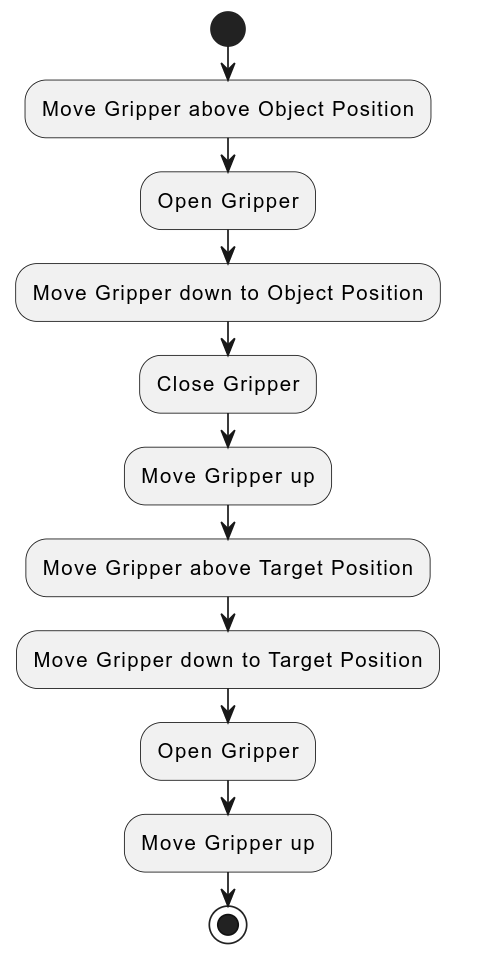
\includegraphics[width=0.5\textwidth]{Figures/pick_place_loop.png}
    \caption{Pick and place implementation}
    \label{fig:pick_n_place}
\end{figure}

\textcolor{red}{ close section } % end red

% \begin{lstlisting}[]%language=plantuml
% @startuml
% start
%     :Move Gripper above Object Position;
%     :Open Gripper;
%     :Move Gripper down to Object Position;
%     :Close Gripper;
%     :Move Gripper up;
%     :Move Gripper above Target Position;
%     :Move Gripper down to Target Position;
%     :Open Gripper;
%     :Move Gripper up;
% stop
% @enduml
% \end{lstlisting}

\textcolor{orange}{
\begin{itemize}
    \item start function used for initialization of the robot controller with the robot as the supervisor and the devices required for the task
    \item loop and autoloop functions containing the actions to be performed by the robot
    \begin{itemize}
      \item loop function contains actions that are not performed in an autonomous way, but controlled by the user. This functions as a manual control loop. This includes the movement of the robot arm and the opening and closing of the gripper. 
      \item autoloop function contains actions that are performed autonomously by the robot. This includes the object detection routine followed by the movement of the robot itself to move the objects from one place to another.
    \end{itemize}
\end{itemize}
} %end orange
